\documentclass{article}

% Language setting
% Replace `english' with e.g. `spanish' to change the document language
\usepackage[english]{babel}

% Set page size and margins
% Replace `letterpaper' with `a4paper' for UK/EU standard size
\usepackage[letterpaper,top=2cm,bottom=2cm,left=3cm,right=3cm,marginparwidth=1.75cm]{geometry}

% Useful packages
\usepackage{amsmath}
\usepackage{graphicx}

\usepackage{graphicx}
\usepackage{caption}
\usepackage{array}
\usepackage{booktabs}
\usepackage{subfig}
\usepackage{amsfonts}
\usepackage{siunitx}
\usepackage{wrapfig}
\graphicspath{ {./images/} }

\title{MIRPR Front Detection}
\author{Gheorghe Mara, Bentea Bogdan, Bogdan Iulian, Bodea Stefan}
\date{}

\begin{document}
\maketitle

\begin{abstract}
Acest proiect are scopul de a cauta fronturile in imaginile meteo.

\end{abstract}

\section{Prima incercare}

Pentru inceput am incercat sa extragem doar fronturile din imagine pentru a simplifica munca clasificatorului. Pentru extragere am folosit biblioteci din cv2 care sa aplice un kernel de diferite dimensiuni pe imagine.

Pentru kernelul {$
  K_{1\times1} =
  \left[  1\right]
$} a rezultat imaginea: 

\begin{figure}[h]
\centering
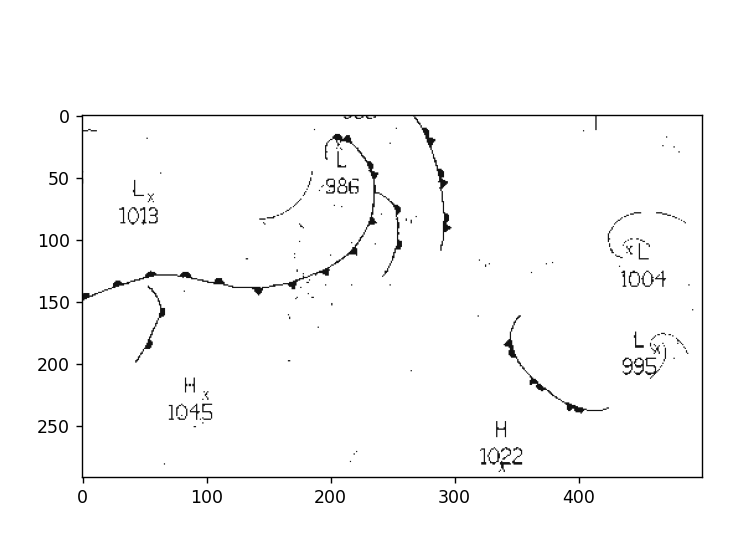
\includegraphics[width=0.5\textwidth]{first.png}
\caption{\label{fig:1}Imaginea rezultata dupa aplicarea kernelului $1\times1$}
\end{figure}

Iar pentru kernelul {$
  K_{2\times2} =
  \left[ {\begin{array}{cc}
    -1 & 1 \\
    1 & -1 \\
  \end{array} } \right]
$} am obtinut: 

\begin{figure}[h]
\centering
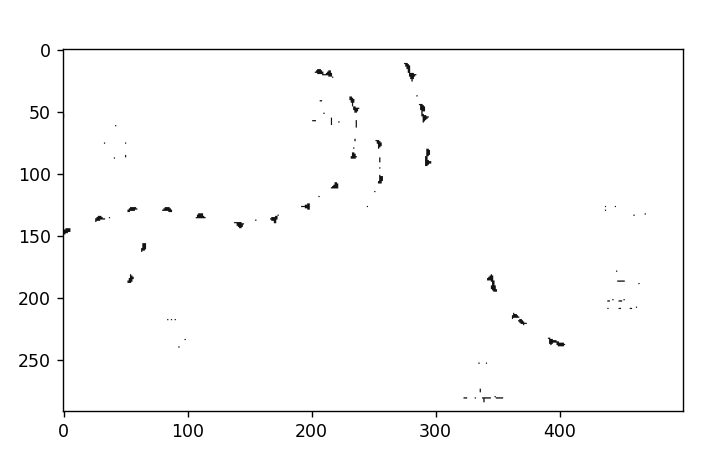
\includegraphics[width=0.5\textwidth]{second.png}
\caption{\label{fig:2}Imaginea rezultata dupa aplicarea kernelului $2\times2$}
\end{figure}

\newpage

\section{Continuarea}

\subsection{Izolare linii}

Pentru a obtine o imagine cat mai "curata", in care sa fie vizibile fronturile, am filtrat imaginile in 2 moduri, cele colore si cele alb negru. 

Pentru cele colore am creat 3 masti, pentru fiecare culoare a fronturilor. O data aplicate mastile, se obtine o imagine cu fundal negru si fronturile colorate. 

In final am transformat imaginea astfel incat sa obtinem fundal alb si fronturi de culoare neagra. Pentru imaginile alb-negru, am incercat sa eliminam acei pixeli negri care au o intensitate mica.

\begin{figure}[!htb]
   \begin{minipage}{0.48\textwidth}
     \centering
     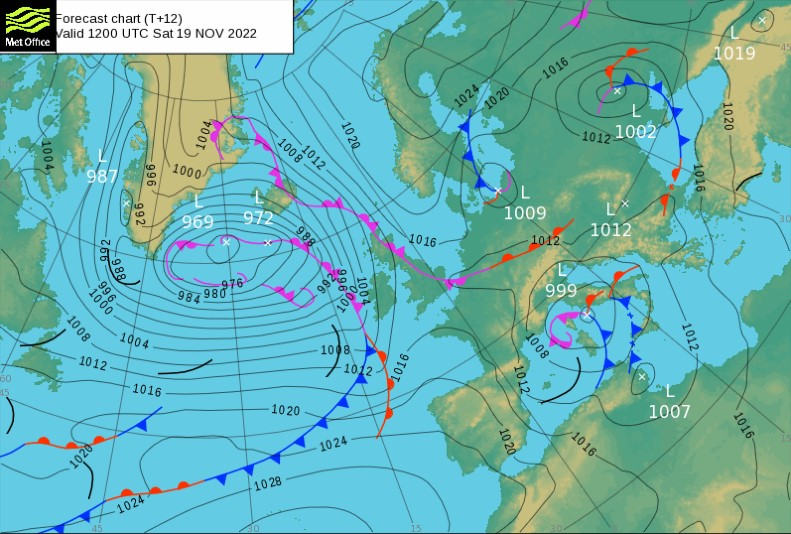
\includegraphics[width=.7\linewidth]{map1.jpg}
     \caption{Map 1}\label{Fig:Data1}
   \end{minipage}\hfill
   \begin{minipage}{0.48\textwidth}
     \centering
     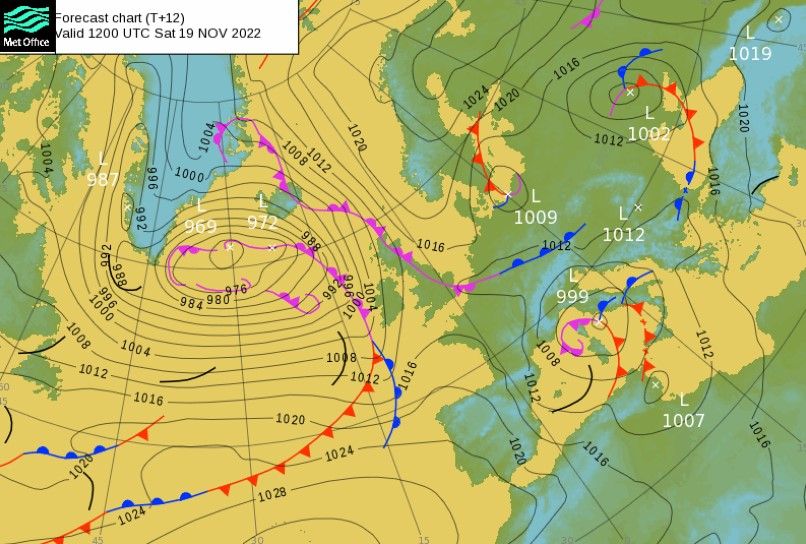
\includegraphics[width=.7\linewidth]{map2.jpg}
     \caption{Map 2}\label{Fig:Data2}
   \end{minipage}
\end{figure}

\begin{figure}[!htb]
   \begin{minipage}{0.48\textwidth}
     \centering
     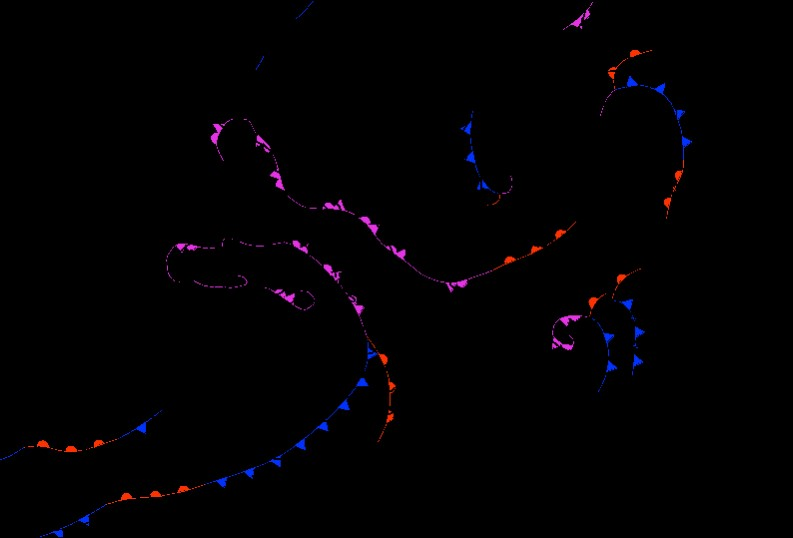
\includegraphics[width=.7\linewidth]{map3.jpg}
     \caption{Map 3}\label{Fig:Data3}
   \end{minipage}\hfill
   \begin{minipage}{0.48\textwidth}
     \centering
     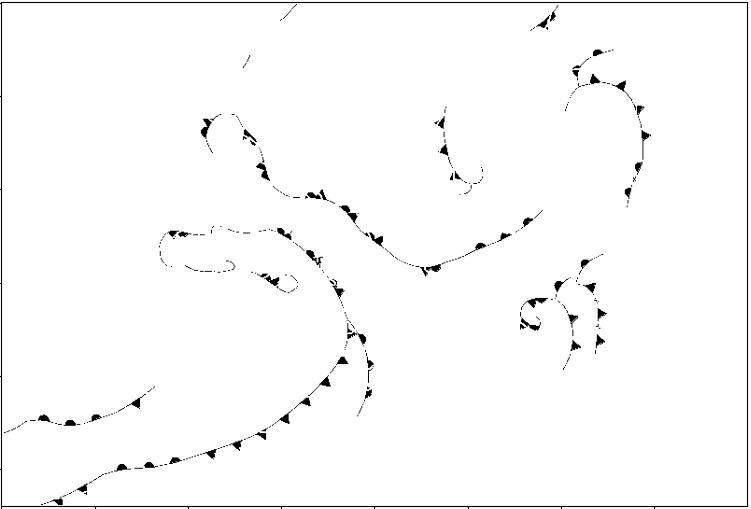
\includegraphics[width=.7\linewidth]{map4.jpg}
     \caption{Map 4}\label{Fig:Data4}
   \end{minipage}
\end{figure}

\begin{figure}[!htb]
   \begin{minipage}{0.48\textwidth}
     \centering
     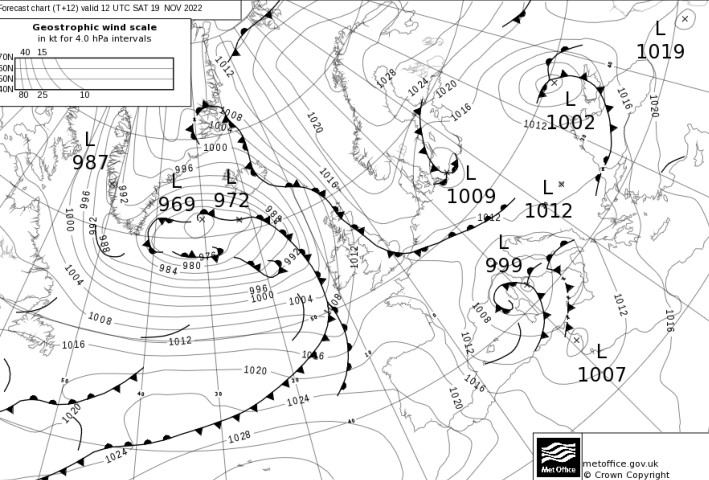
\includegraphics[width=.7\linewidth]{map5.jpg}
     \caption{Map 5}\label{Fig:Data5}
   \end{minipage}\hfill
   \begin{minipage}{0.48\textwidth}
     \centering
     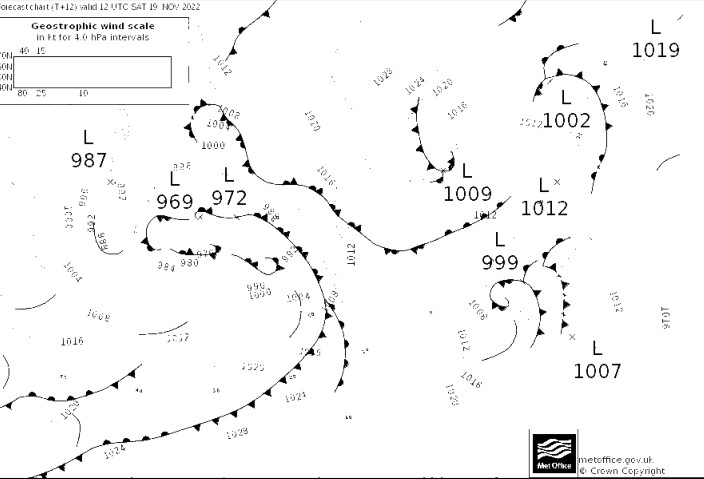
\includegraphics[width=.7\linewidth]{map6.jpg}
     \caption{Map 6}\label{Fig:Data6}
   \end{minipage}
\end{figure}

\subsection{Creare si antrenare model}

Am creat un model de tipul Sequential cu urmatoarele layere:
\begin{enumerate}
  \item Rescaling, pentru a normaliza pixeli care primeste ca si input o poza de dimensiunile (50, 50, 3)
  \item Un layer de convolutie cu 16 kerneluri urmat de MaxPooling.
  \item Un layer de convolutie cu 32 de kerneluri si MaxPooling.
  \item Un layer de convolutie cu 64 de kerneluri si MaxPooling.
  \item Un layer de Flatten dupa care incepe partea de componenta conexa completa care are pe primul strat 128 de noduri.
  \item Un layer de 3 noduri reprezentand nodurile de iesire.
\end{enumerate}

Pentru a compila modelul am folosit optimizer-ul 'adam' si metrica de acuratete.

Am antrenat modelul pentru a putea recunoaste fronturile cold, warm si occluded.
A primit ca si date de antrenament crop-uri din imaginile reale ale acestor date.

Ca si acuratete a ajuns la 0.7 pentru datele de validare.
Dupa care parcurgem imaginea filtrata si verificam fiecare patrat de dimensiunile (50, 50, 3) pe care-l clasificam cu modelul, daca modelul il clasifica "sigur" ca un anume tip de front atunci acel patrat este considerat un anume tip de front.
    
\begin{figure}[h]
\centering
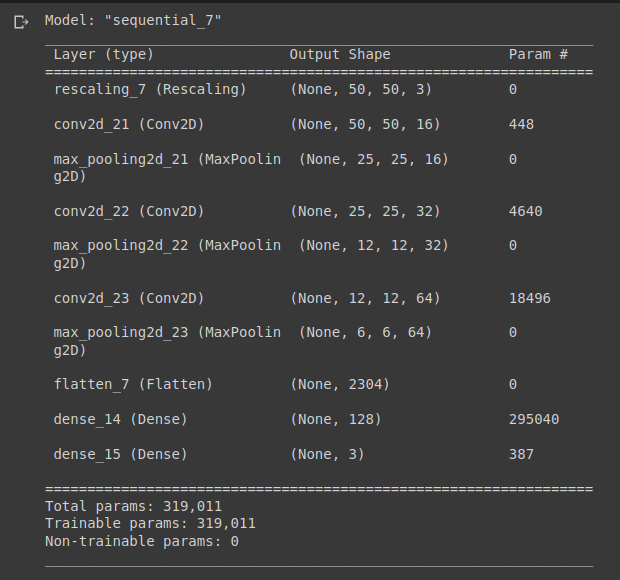
\includegraphics[width=0.5\textwidth]{model1.jpg}
\caption{\label{fig:3}Model de tip Sequential}
\end{figure}

\begin{figure}[h]
\centering
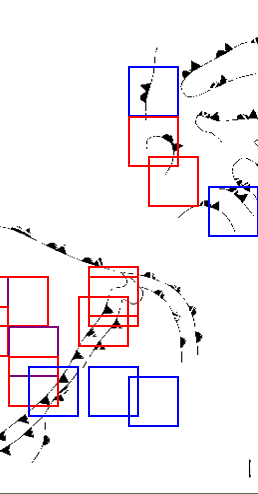
\includegraphics[width=0.5\textwidth]{result1.jpg}
\caption{\label{fig:4}Rezultat 1}
\end{figure}

\begin{figure}[!htb]
   \begin{minipage}{0.30\textwidth}
     \centering
     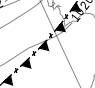
\includegraphics[width=.7\linewidth]{result2.jpg}
     \caption{Rezultat 2}\label{Fig:Rez2}
   \end{minipage}\hfill
   \begin{minipage}{0.30\textwidth}
     \centering
     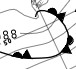
\includegraphics[width=.7\linewidth]{result3.jpg}
     \caption{Rezultat 3}\label{Fig:Rez3}
   \end{minipage}
   \begin{minipage}{0.30\textwidth}
     \centering
     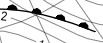
\includegraphics[width=.7\linewidth]{result4.jpg}
     \caption{Rezultat 4}\label{Fig:Rez4}
   \end{minipage}
\end{figure}

\clearpage
\section{Imbunatatirea algoritmului}

\subsection{Metodologie}
  Folosim un model pre-antrenat, numit VGG-16. Acest model a fost propus de Karen Simonyan si Andrew Zisserman, membri ai "Visual Geometry Group" din cadrul Univerisatii Oxford. 
  VGG-16 atinge acuratete de pana la 92.7\% pe setul de date ImageNet (ce contine peste 14 milioane de imagini, ce apartin de 1000 de clase).
  \newline
  In cazul algoritmului nostru, am adaugat trei layere fully connected, unul cu 1024 de noduri, urmatorul cu 512 si ultimul cu 4 noduri, egal cu numarul de clase.
  Am modificat modelul VGG-16 pentru a clasifica 4 clase pe care le gasim in pozele cu fronturile, adica clasa "COLD" care este reprezentata de simbolul triunghi, clasa "WARM" care este reprezentata de simbolul semicerc, clasa "OCCLUDED" care este reprezentata de cele doua simboluri alaturate si clasa "WHITE" care reprezinta tot ce nu este una din cele trei clase de interes. 
  \bigskip
  
  \begin{figure}[!htb]
  \centering
  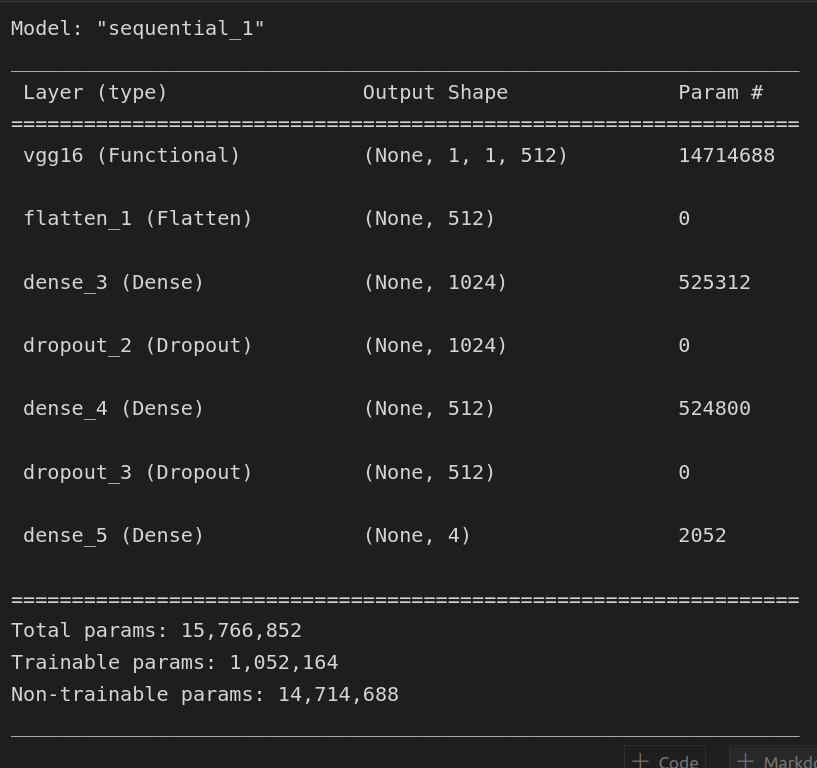
\includegraphics[width=0.8\textwidth]{result5.jpg}
  \caption{\label{fig:6}Model de tip VGG-16}
  \end{figure}

  \newpage
  Pentru a obtine o clasificare mai buna, am decis sa impartim imaginea filtrata in zone de dimensiune mai mica, adica imagini de 32x32 px, fata de la prima versiune unde imaginile aveau dimensiunea de 100x100 px.
  O imagine acum contine un singur simbol (Figurile 15 - 23), nu o linie cu un sir de simboluri.
  
  \begin{figure}[!htb]
    \begin{minipage}{0.3\textwidth}
      \centering
      
\includegraphics[width=.35\linewidth]{cold1.png}
      \caption{Cold symbol}\label{Fig:Cold1}
    \end{minipage}\hfill
    \begin{minipage}{0.3\textwidth}
      \centering
      
\includegraphics[width=.35\linewidth]{cold2.png}
      \caption{Cold symbol}\label{Fig:Cold2}
    \end{minipage}
    \begin{minipage}{0.3\textwidth}
      \centering
      
\includegraphics[width=.35\linewidth]{cold3.png}
      \caption{Cold symbol}\label{Fig:Cold3}
    \end{minipage}
 \end{figure}
 
 \begin{figure}[!htb]
  \begin{minipage}{0.3\textwidth}
    \centering
    
\includegraphics[width=.35\linewidth]{warm1.png}
    \caption{Warm symbol}\label{Fig:Warm1}
  \end{minipage}\hfill
  \begin{minipage}{0.3\textwidth}
    \centering
    
\includegraphics[width=.35\linewidth]{warm2.png}
    \caption{Warm symbol}\label{Fig:Warm2}
  \end{minipage}
  \begin{minipage}{0.3\textwidth}
    \centering
    
\includegraphics[width=.35\linewidth]{warm3.png}
    \caption{Warm symbol}\label{Fig:Warm3}
  \end{minipage}
\end{figure}
 
\begin{figure}[!htb]
  \begin{minipage}{0.3\textwidth}
    \centering
    
\includegraphics[width=.35\linewidth]{occluded1.png}
    \caption{Occluded symbol}\label{Fig:Occluded1}
  \end{minipage}\hfill
  \begin{minipage}{0.3\textwidth}
    \centering
    
\includegraphics[width=.35\linewidth]{occluded2.png}
    \caption{Occluded symbol}\label{Fig:Occluded2}
  \end{minipage}
  \begin{minipage}{0.3\textwidth}
    \centering
    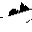
\includegraphics[width=.35\linewidth]{occluded3.png}
    \caption{Occluded symbol}\label{Fig:Occluded3}
  \end{minipage}
\end{figure}

Am avut doua iteratii ale modelului inainte de aceasta unde am folosit, o data imaginile mai mari in varianta color si in varianta alb-negru.
In variantele anterioare, imaginile nu contineau un singur simbol ci mai multe de acelasi tip. (Figurile 24 - 29).

\begin{figure}[!htb]
  \begin{minipage}{0.32\textwidth}
    \centering
    \includegraphics[width=.33\linewidth]{cold_v1.png}
    \caption{Cold b\&w}\label{Fig:ColdV1}
  \end{minipage}
  \begin{minipage}{0.35\textwidth}
    \centering
    \includegraphics[width=.35\linewidth]{warm_v1.png}
    \caption{Warm b\&w}\label{Fig:WarmV1}
  \end{minipage}
  \begin{minipage}{0.32\textwidth}
    \centering
    \includegraphics[width=.33\linewidth]{occluded_v1.png}
    \caption{Occluded b\&w}\label{Fig:OccludedV1}
  \end{minipage}
\end{figure}

\begin{figure}[!htb]
  \begin{minipage}{0.32\textwidth}
    \centering
    \includegraphics[width=.33\linewidth]{cold_v2.png}
    \caption{Cold color}\label{Fig:ColdV1}
  \end{minipage}
  \begin{minipage}{0.35\textwidth}
    \centering
    \includegraphics[width=.35\linewidth]{warm_v2.png}
    \caption{Warm color}\label{Fig:WarmV1}
  \end{minipage}
  \begin{minipage}{0.32\textwidth}
    \centering
    \includegraphics[width=.33\linewidth]{occluded_v2.png}
    \caption{Occluded color}\label{Fig:OccludedV1}
  \end{minipage}
\end{figure}

\newpage


\subsection{Analiza comparative}
\bigskip
{\centering
\begin{tabular}{c || c c c} \toprule
    {} & {Varianta 1} & {Varianta 2} & {Varianta 3} \\ \midrule
    {Acuratete} & 0.7251 & 0.6571 & 0.8750 \\
    {Timpi de inferenta (ms)} & 3511.568115 & 3349.47949 & 2775.35156 \\
    {Matricea de confuzie} & {Figura 30} & {Figura 31} & {Figura 32} \\
    {Experiment} & {Figura 33} & {Figura 34} & {Figura 35} \\
\end{tabular}\par}
\bigskip
  \begin{figure}[!htb]
    \begin{minipage}{0.45\textwidth}
      \centering
      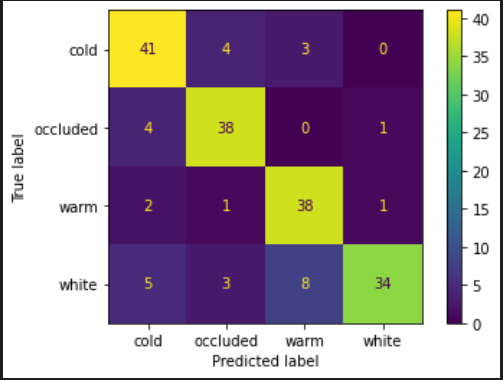
\includegraphics[width=1\linewidth]{model_v1_colored_confusion_matrix.png}
      \caption{Matricea de confuzie pentru varianta 1}\label{Fig:Cold1}
    \end{minipage}\hfill
    \begin{minipage}{0.45\textwidth}
      \centering
      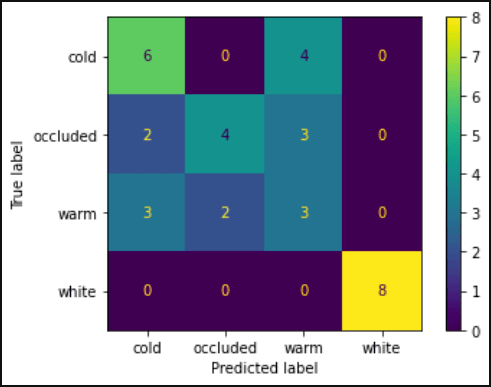
\includegraphics[width=1\linewidth]{model_v2_bw_confusion_matrix.png}
      \caption{Matricea de confuzie pentru varianta 2}\label{Fig:Cold2}
    \end{minipage}
 \end{figure}

 \begin{figure}[!htb]
  \centering
  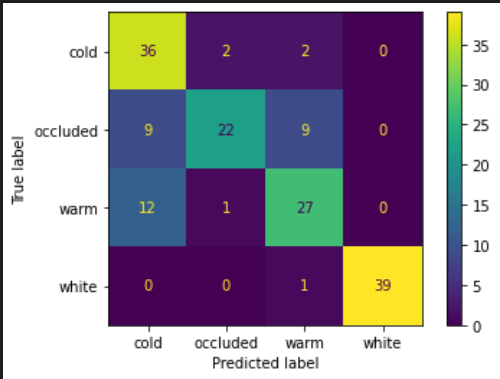
\includegraphics[width=0.45\textwidth]{model_v3_confusion_matrix.png}
  \caption{Matricea de confuzie pentru varianta 3}
\end{figure}

\newpage
  \begin{figure}[!htb]
    \begin{minipage}{0.45\textwidth}
      \centering
      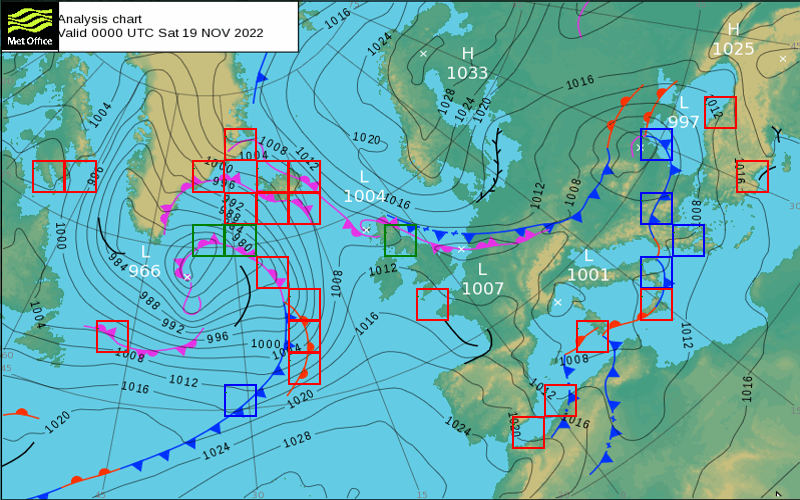
\includegraphics[width=1\linewidth]{model_v1_colored_output.png}
      \caption{Experiment varianta 1}\label{Fig:Cold1}
    \end{minipage}\hfill
    \begin{minipage}{0.45\textwidth}
      \centering
      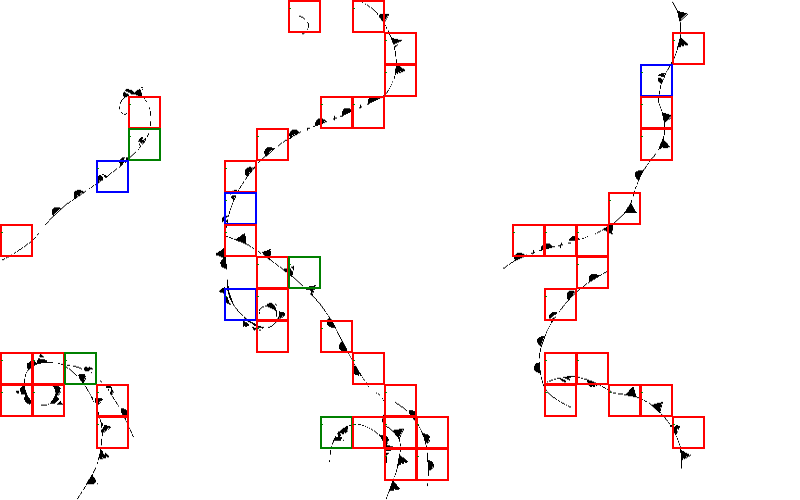
\includegraphics[width=1\linewidth]{model_v2_bw_output.png}
      \caption{Experiment varianta 2}\label{Fig:Cold2}
    \end{minipage}
 \end{figure}

 \begin{figure}[!htb]
  \centering
  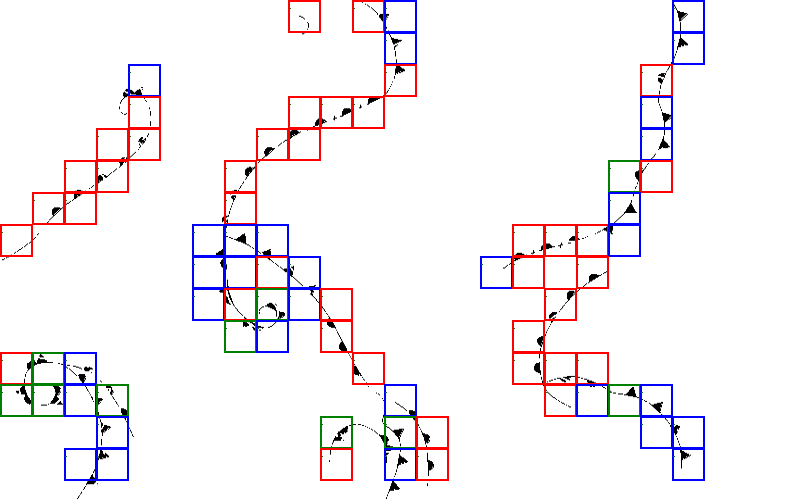
\includegraphics[width=0.45\textwidth]{model_v3_output.png}
  \caption{Experiment varianta 3}
\end{figure}

\subsection{Rezultate}

\bigskip
\centering
\begin{tabular}{c || c c c c} \toprule
    {Metrica} & {Cold} & {Warm} & {Occluded} & {White} \\ \midrule
    {Precizia} & 0.54 & 0.64 & 0.80 & 0.97 \\
    {Rapelul} & 0.93 & 0.45 & 0.50 & 0.97 \\
\end{tabular}

\bigskip
Pentru versiunea 3 acuratetea obtinuta este aproximativ 87\% pe datele de validare iar pe un exemplu real modelul se descurca cam asa.
\bigskip

 \begin{figure}[!htb]
  \centering
  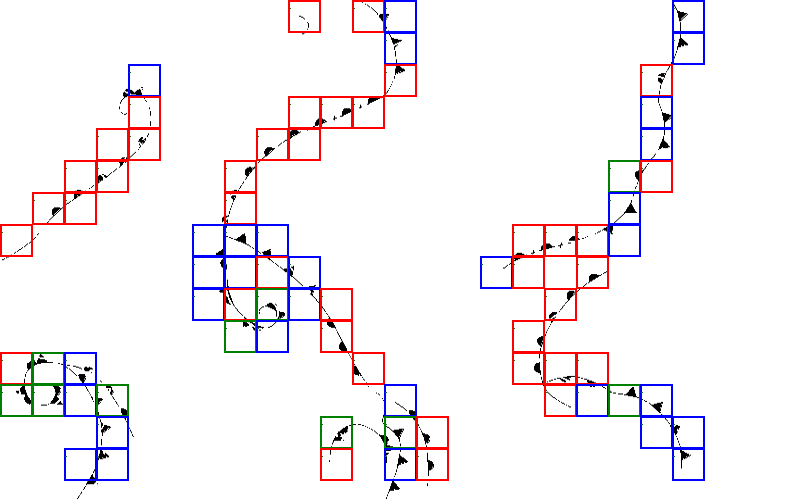
\includegraphics[width=0.6\textwidth]{model_v3_output.png}
  \caption{Experiment varianta 3}
\end{figure}

\end{document}